% P05 diagnostic figure paired_domains|C-RANDOM-FOREST|M01; allowlisted public aggregate points.
% Each point is an aggregate mean or bin over repeated contexts, not an independent sample.
% data_sha256=7f60e425b5fe235c362c21442c3237e1521aad33df8bebdebfd5854e0cfadd4b
\documentclass[tikz,border=5pt]{standalone}
\ifdefined\pdfinfoomitdate\pdfinfoomitdate=1\fi
\ifdefined\pdfsuppressptexinfo\pdfsuppressptexinfo=-1\fi
\ifdefined\pdftrailerid\pdftrailerid{}\fi
\usepackage{pgfplots}
\usepgfplotslibrary{groupplots}
\pgfplotsset{compat=1.18}
\definecolor{p05Blue}{HTML}{0072B2}
\definecolor{p05Orange}{HTML}{E69F00}
\definecolor{p05Green}{HTML}{009E73}
\definecolor{p05Purple}{HTML}{CC79A7}
\definecolor{p05Red}{HTML}{D55E00}
\definecolor{p05Sky}{HTML}{56B4E9}
\begin{document}
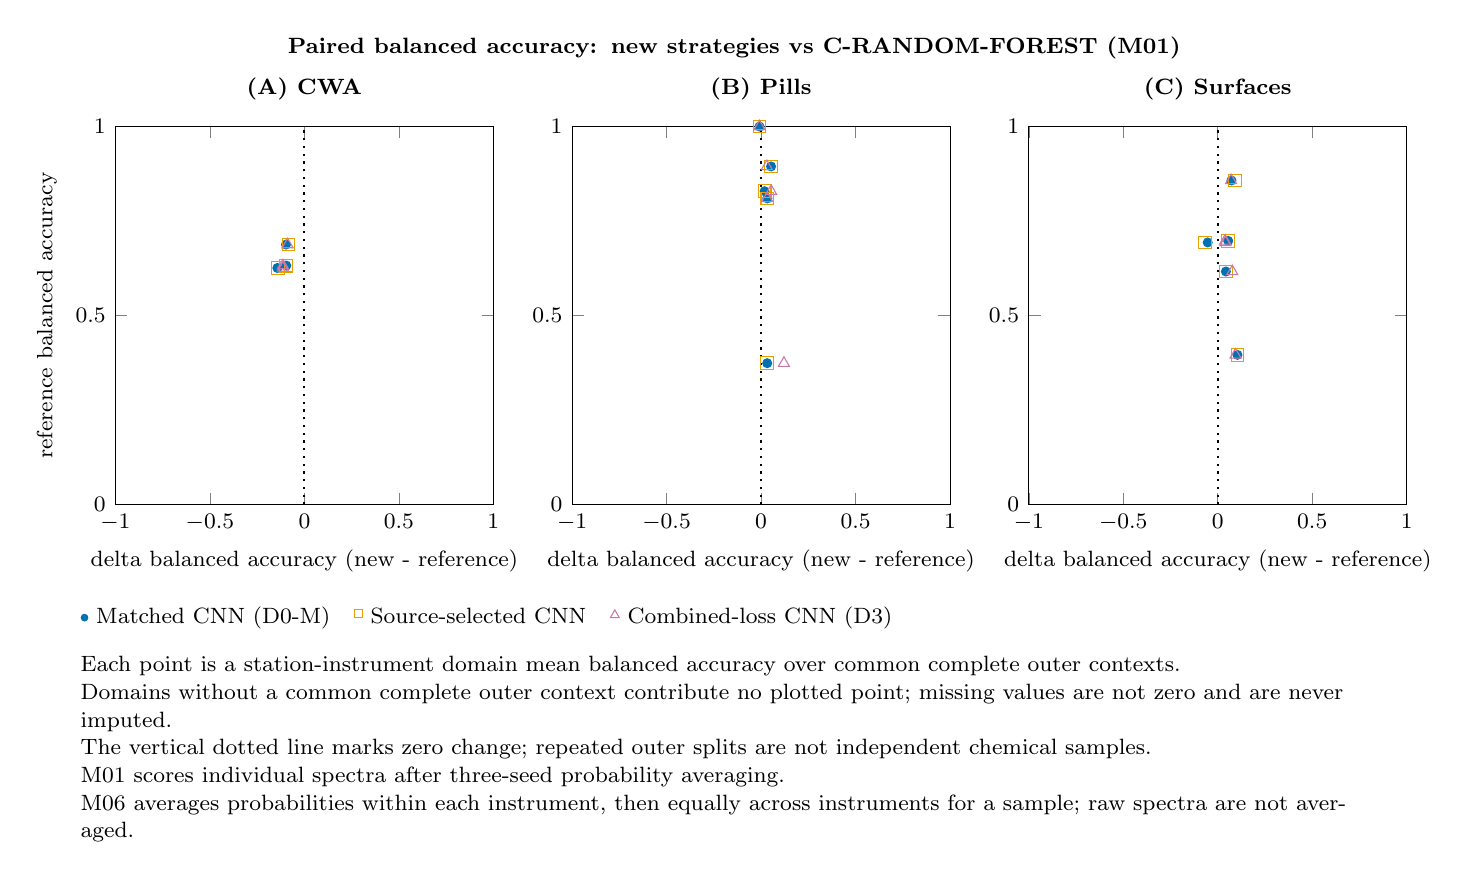
\begin{tikzpicture}
\begin{groupplot}[
  group style={group size=3 by 1, horizontal sep=1.0cm, vertical sep=1.8cm},
  width=4.8cm, height=4.8cm, scale only axis,
  xmin=-1, xmax=1, ymin=0, ymax=1,
  xtick={-1,-0.5,0,0.5,1}, ytick={0,0.5,1},
  tick label style={font=\fontsize{8}{10}\selectfont, color=black},
  label style={font=\fontsize{8}{10}\selectfont, color=black},
  title style={font=\fontsize{8}{10}\selectfont\bfseries, color=black},
]
\nextgroupplot[title={(A) CWA}, xlabel={delta balanced accuracy (new - reference)}, ylabel={reference balanced accuracy}]
\addplot[black, dotted, line width=0.8pt] coordinates {(0,0) (0,1)};
\addplot[only marks, mark=*, mark size=1.6pt, color=p05Blue, mark options={fill=p05Blue, draw=p05Blue}] coordinates {(-0.1429232804232804,0.62582010582010572) (-0.097380952380952374,0.68777777777777782) (-0.09582431457431459,0.63215307840307833)};
\addplot[only marks, mark=square, mark size=2.3pt, color=p05Orange, mark options={fill=none, draw=p05Orange}] coordinates {(-0.14093915343915342,0.62582010582010572) (-0.09582431457431459,0.63215307840307833) (-0.084325396825396831,0.68777777777777782)};
\addplot[only marks, mark=triangle, mark size=2.3pt, color=p05Purple, mark options={fill=none, draw=p05Purple}] coordinates {(-0.11362433862433859,0.62582010582010572) (-0.1136219336219336,0.63215307840307833) (-0.088769841269841249,0.68777777777777782)};
\nextgroupplot[title={(B) Pills}, xlabel={delta balanced accuracy (new - reference)}]
\addplot[black, dotted, line width=0.8pt] coordinates {(0,0) (0,1)};
\addplot[only marks, mark=*, mark size=1.6pt, color=p05Blue, mark options={fill=p05Blue, draw=p05Blue}] coordinates {(-0.0083333333333333315,1) (0.018611111111111099,0.82888888888888901) (0.032440476190476186,0.37392857142857139) (0.033472222222222209,0.80984126984126981) (0.052777777777777792,0.89444444444444449)};
\addplot[only marks, mark=square, mark size=2.3pt, color=p05Orange, mark options={fill=none, draw=p05Orange}] coordinates {(-0.0083333333333333315,1) (0.018611111111111099,0.82888888888888901) (0.032440476190476186,0.37392857142857139) (0.033472222222222209,0.80984126984126981) (0.052777777777777792,0.89444444444444449)};
\addplot[only marks, mark=triangle, mark size=2.3pt, color=p05Purple, mark options={fill=none, draw=p05Purple}] coordinates {(-0.0083333333333333315,1) (0.030555555555555575,0.89444444444444449) (0.032222222222222194,0.80984126984126981) (0.053333333333333344,0.82888888888888901) (0.12102513227513227,0.37392857142857139)};
\nextgroupplot[title={(C) Surfaces}, xlabel={delta balanced accuracy (new - reference)}]
\addplot[black, dotted, line width=0.8pt] coordinates {(0,0) (0,1)};
\addplot[only marks, mark=*, mark size=1.6pt, color=p05Blue, mark options={fill=p05Blue, draw=p05Blue}] coordinates {(-0.053134920634920625,0.69341269841269837) (0.043021885521885544,0.61650312650312644) (0.05527777777777778,0.69738095238095232) (0.072341269841269817,0.85730158730158745) (0.10416666666666666,0.39583333333333331)};
\addplot[only marks, mark=square, mark size=2.3pt, color=p05Orange, mark options={fill=none, draw=p05Orange}] coordinates {(-0.066468253968253954,0.69341269841269837) (0.044225589225589237,0.61650312650312644) (0.05527777777777778,0.69738095238095232) (0.09198412698412696,0.85730158730158745) (0.10416666666666666,0.39583333333333331)};
\addplot[only marks, mark=triangle, mark size=2.3pt, color=p05Purple, mark options={fill=none, draw=p05Purple}] coordinates {(0.038749999999999993,0.69738095238095232) (0.040476190476190478,0.69341269841269837) (0.070555555555555524,0.85730158730158745) (0.076931818181818185,0.61650312650312644) (0.093888888888888883,0.39583333333333331)};
\end{groupplot}
\node[anchor=south, font=\fontsize{8}{10}\selectfont\bfseries, color=black, align=center, text width=16.6cm] at (current bounding box.north) {Paired balanced accuracy: new strategies vs C-RANDOM-FOREST (M01)};
\node[anchor=north, font=\fontsize{8}{10}\selectfont, color=black, align=left, text width=16.6cm] (p05legend) at ([yshift=-2mm]current bounding box.south) {\tikz[baseline=-0.6ex]\fill[p05Blue](0,0)circle(1.4pt);\ Matched CNN (D0-M)\quad \tikz[baseline=-0.6ex]\draw[p05Orange](0,0)rectangle(2.8pt,2.8pt);\ Source-selected CNN\quad \tikz[baseline=-0.6ex]\draw[p05Purple](0,0)--(1.6pt,2.8pt)--(3.2pt,0)--cycle;\ Combined-loss CNN (D3)};
\node[anchor=north, font=\fontsize{8}{10}\selectfont, color=black, align=left, text width=16.6cm] at ([yshift=-1mm]p05legend.south) {Each point is a station-instrument domain mean balanced accuracy over common complete outer contexts.\\Domains without a common complete outer context contribute no plotted point; missing values are not zero and are never imputed.\\The vertical dotted line marks zero change; repeated outer splits are not independent chemical samples.\\M01 scores individual spectra after three-seed probability averaging.\\M06 averages probabilities within each instrument, then equally across instruments for a sample; raw spectra are not averaged.};
\end{tikzpicture}
\end{document}
